\documentclass{llncs}
\usepackage{makeidx}
\usepackage[pdftex]{hyperref}
\usepackage{pdfpages}
\usepackage{listings}
\usepackage{graphicx}

\begin{document}

\pagestyle{headings}
\title{The road to a Building Automation DSL through MDD}
\titlerunning{Building Policy Engine}
\author{Hansen, K.\, Kontostathis, K., Schmidt, E.}
\authorrunning{Hansen, K et al.}
\tocauthor{Hansen, K., Kontostathis, K., Schmidt, E.}
\institute{IT-University of Copenhagen, Denmark,\\
\email{kben@itu.dk}, \email{kkon@itu.dk}, \email{eker@itu.dk}}
\maketitle

\vspace{-0.3cm}

\begin{abstract}
Modern buildings often consist of many different types of sensors and actuators. It is a complex task to control and manage them, especially when aiming for optimal energy efficiency and human comfort. If easily specified automated control of buildings is achievable, the result would be reduction of energy usage and natural resources like gas and water. We specified a building's automation Domain Specific Language (DSL) based on requirements obtained from interviews with several large companies, and built it using Eclipse Modeling Framework and XText. The DSL is validated by implementing all the discovered policies.
\end{abstract}

\vspace{-0.5cm}

\section{Introduction}
Energy and natural resources are precious commodities. In~\cite{janssen2004towards} it is stated that residential buildings use about 89\% of the total energy consumption for space heating, cooling and water heating. Electrical appliances use 11\%. Other buildings use 79\% of the total energy consumption for space heating, cooling, water heating and lighting. To \textit{manually} control buildings for energy efficiency and optimal human comfort is a time-consuming and inefficient task, if even possible. The controller needs to possess a diverse knowledge of the necessary equipment and the building's characteristics at the same time. Modern buildings today often come equipped with a suite of sensors and actuators, opening up for a degree of customizable control. Building automation is therefore not only possible, but also necessary. \textit{``Worldwide, there is no doubt that efficient energy saving is only possible with modern BA based on networking in all levels of abstraction."}~\cite{dietrich2010communication}. Constructing resource efficient buildings makes sense, both in a political and economical perspective. 

Consequently, our collective need is the adaptation of buildings to the users and the sensor-perceived environment. This can be achieved by developing governing \textit{policies} (defined as pieces of code) based on input such as semi-static data, dynamic data and sensor input, which control the actuators and thereby leading to the desired building state.

Merriam-Webster defines \textit{policy} as ``a definite course or method of action selected from among alternatives and in light of given conditions to guide and determine present and future decisions."

For this paper, many companies were interviewed regarding their need for building automation \textit{policies}. After analyzing the interviews and iteratively specifying a DSL for building automation, we argue by example, that our proposed DSL can actually satisfy the needs and the intended requests made during the interviews.

The structure of the paper is as follows. We start by discussing all \nameref{sec:relatedwork} and compare it with our own. We then move on to~\nameref{sec:method}, followed by a section on~\nameref{sec:dsldesign}. Later on we explain our~ \nameref{sec:evaluation}, and its results in the~\nameref{sec:discussion} section. Last comes the summing up of our findings in~\nameref{sec:conclusion}.

\section{Related work}\label{sec:relatedwork}
A lot of research has already been conducted in home and building automation, spanning from low level communication protocols like BACnet, LonWorks and EIB/KNX~\cite{communication} to full system implementations. In comparison, less progress has been made on user friendly DSL designs, where everyday building concepts are mixed with time constraints and conditional logic for building automation. 

In~\cite{smartscript} a DSL named SmartScript is developed. Based on a publish/subscribe paradigm it is intended for appliance control, and implemented with a KNX adapter. It allows grouping of devices in order to make possible for instance to turn on the light and dim it using the same `light' concept, even though the light switch and dimmer are two separate electronic components. The language features three types of statements; Action, If and Loop. Specifically, there are two actions; Set and Get. Although it is possible to use the group concept, it does not seem to be possible to define the entire building with rooms based on different types. This results in a long collection of variables, even for small and simple buildings. Moreover, the script seems to be operating on a much lower abstraction level than our DSL, maybe due to its implementation that seems to have pulled the DSL more into the direction of a GPL. 

In~\cite{habitation} there is a clear distinction between usage of the domain experts (called the Catalog View) and the domain users (called the Application view). A graphical editor is used when designing an application, by dragging and dropping types into flows that will be orderly executed. However, the user designing the application still has to get familiar with concepts such as \textit{standard functional units}, \textit{FUnitLinks} and \textit{Scenes}. Again, our DSL is at a higher abstraction level. However, the catalog view might be considered as the current state of our metamodel, where the different concepts are defined. Our model only operates on concepts already known to people expected to work with building automation like \textit{Building, Floor, Room, Sensor, Actuator, Schedule, and Policy}. Apart from the obvious differences, our DSL is text-based, versus the graphical editor in Habitation, our flow resides in the combinatory logic derived from time schedules, room types, boolean states and conditional logic specified in the policies. This will become evident in the \nameref{sec:dsldesign} section.

In the Google sponsored Home Automation Bus - openHab~\cite{openhab} it is also possible to specify rules, running on actual implemented hardware. OpenHAB offers a whole suite of implemented protocol standards and functionalities, that includes an Xtext based script interpreter. OpenHAB's rule language is, like most other systems, very low level and does not offer the expressive benefits of a high abstraction DSL.

\section{Method}\label{sec:method}
We have tailored our method as follows;

\begin{enumerate}
	\item Interviews and analysis: We conducted open-ended interviews with people working in, or close, to FM in various danish companies.
	\item Design and development: We designed a building automation policy DSL based on our analysis of the interviews
	\item Evaluation: We evaluated the DSL in two ways;
	\begin{enumerate}
		\item By asking our interviewees to have a look at our DSL (not sure!) and fill out a questionnaire
		\item By conducting sessions where students had to write different policies, and then analyzing their behavior
	\end{enumerate}
\end{enumerate}

\section{Interviews and analysis}\label{sec:interviews}
Since building control resides with Facility Management we found it pertinent to interview company employees working on or close to that field. We conducted open-ended interviews with these companies and documented their content mostly by handwritten notes or in some rare cases by audio record. The main purpose of the interviews was to document;

\begin{enumerate}
	\item existing governing rules, implicit or explicit.
	\item existing and requested, sensors and actuators.
	\item requests for new governing rules regardless of their practicality or feasibility.
\end{enumerate}

In order to gather enough material to conceptualize a proper DSL, we interviewed people from the following companies; Br\"{u}el \& Kj\ae r, Bygningsstyrelsen, IT-University of Copenhagen, K\o benhavns Tekniske Skole, ST Aerospace - Denmark and UNI-C.

While conducting the interviews, we pointed out that practicality or feasibility should not influence the requests for new governing rules. This proved hard for the interviewees. Some interviews were therefore conducted over several sessions, giving the interviewees time to think creatively. 

We only used natural language (English, Danish) to give examples of existing building policies and facilitate the discovery of new, relevant ones. This was done to avoid the limitations of technology, like the expressiveness of a programming language.

Finally, this project is based on the requirements defined by the professionals working in Facility Management, and used their stated policies as requirements to be implemented as grammar-passed code using the developed DSL.

\section{Design and development}\label{sec:dsldesign}
By using Eclipse~\cite{eclipse}, EMF~\cite{emf} and Xtext~\cite{xtext} we built a domain specific language that is rich enough to express the policies discovered in the analysis. We developed a grammar that is based on our programming experience, and believed to have a consistent forthcoming syntax and conceptual constructs. Finally, we used our Policy Engine DSL editor to write the policies.

Our model is of considerable size, and consists of the following core packages, differentiated in separate Ecore Diagrams (can be viewed in full in \nameref{sec:appendix-a}); 9 sensors classes, 6 actuators classes, 6 expression language classes, 5 building definition classes and 10 policy definition classes.

We have included the full DSL implementation of one of the interviewees, Br\"{u}el \& Kj\ae r in Appendix [INSERT APPENDIX HERE]. Please note that this is a fully working implementation that is running in Eclipse.

\subsubsection{Sensors}:
\begin{figure}
	\centering
    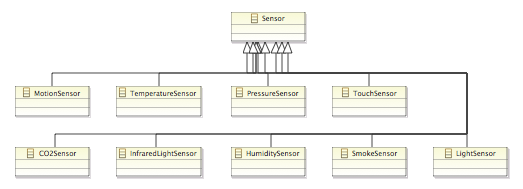
\includegraphics[scale=0.7]{ecore-sensors.png} 
	\caption{An example of \textit{Sensors} defined for a interviewee.}
	\label{fig:ecore-sensors}
\end{figure}

\pagebreak
\subsubsection{Actuators}:
\begin{figure}
	\centering
    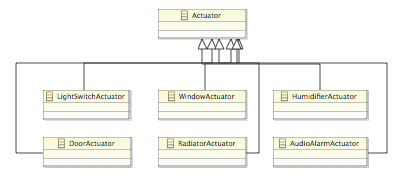
\includegraphics[scale=0.7]{ecore-actuators.png}   
	\caption{An example of \textit{Actuators} defined for a interviewee.}
	\label{fig:ecore-actuators}
\end{figure}

\subsubsection{Expression language}:
\begin{figure}
  \centering
    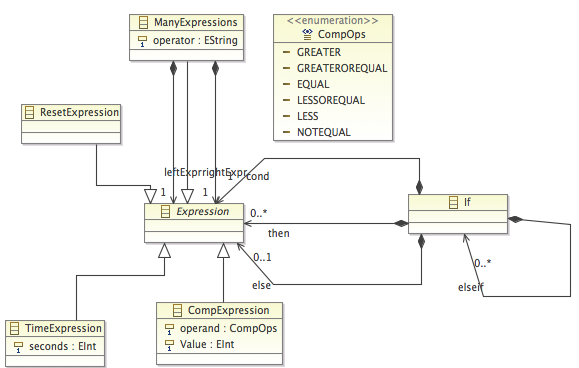
\includegraphics[width=10cm]{ecore-expression-language.png} 
	\caption{An example of \textit{expression language} defined for a interviewee.}
	\label{fig:ecore-expression-language}
\end{figure}

\pagebreak
\subsubsection{Building definition}:
\begin{figure}
  \centering 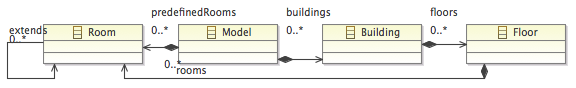
\includegraphics[scale=0.4]{ecore-building-definition.png}  
	\caption{The Metamodel related to the \textit{building definition}. The inherited class NamedElement has been omitted.}
	\label{fig:ecore-building-definition}
\end{figure}

\subsubsection{Policy definition}:
\begin{figure}
  \centering
    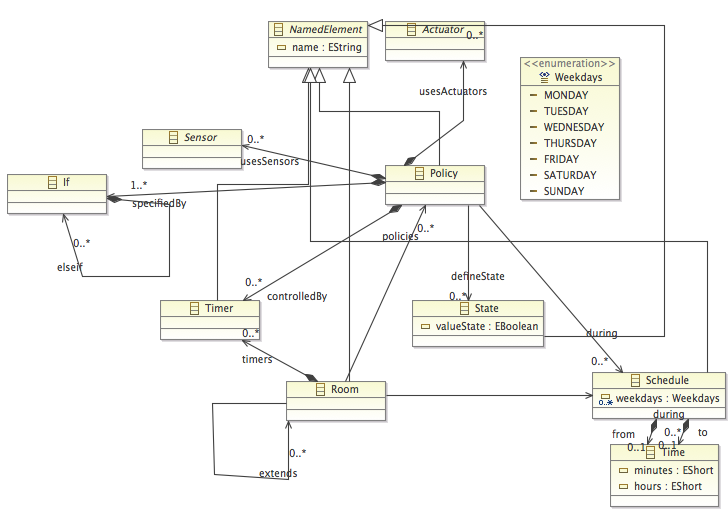
\includegraphics[scale=0.3]{ecore-policy-definition.png}	
	\caption{An example of \textit{policy definition} defined for a interviewee.}
	\label{fig:ecore-policy-definition}
\end{figure}

\pagebreak
There are several extra classes, consisting of subsystems that can be implemented in future work.

During the analysis of the interviews, different meta-constructs were defined. It was evident that the below three key concepts were needed in order to tailor the policies for the interviewees using the DSL;

\begin{enumerate}
	\item \textit{Time}. Time has to be an integral part of the DSL, and not just related with the internal policy logic. Several interviewees mention concepts like weekdays, weekends, normal working hours, holidays, night, day, morning etc.
	
	\item \textit{Building specification}. It should be possible to define the buildings, their floors, number and types of rooms etc.

	\item \textit{Policy}. The actual behavior, ie. adjusting actuators based on sensor input, needs to be defined. 
\end{enumerate}

\subsection{Time}\label{subsec:time}
The analysis of the interviews clearly shows that Time is necessary. We have extrapolated the need for Time in two different cases;
	\begin{enumerate}
		\item Time conditional expression - an expression used for determining the flow of a behavior.
		\item Schedules - types that define a timespan which can later be attached to a specific behavior.
	\end{enumerate}

\subsubsection{Time conditional expression}\label{subsubsec:conditionalexpression}
A \textit{time conditional expression} is an `if' statement that can react based on a built-in timer function. 

\begin{figure}
  \centering
    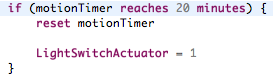
\includegraphics[scale=.6]{dsl-conditional-time-expression.png} 
	\caption{An example of a \textit{time conditional expression} that evaluates to true if more than 20 minutes have passed.}
	\label{fig:dsl-conditionalexpression}
\end{figure}

\newpage
\subsubsection{Schedules}\label{subsubsec:schedules}
\textit{Schedules} are predefined types representing a timespan where action or no-action takes place. The \textit{Schedules} can overlap, resulting in the flexibility of many policies being run in succession, which was the common request of (almost) all interviewees.

\begin{figure}
  	\centering
    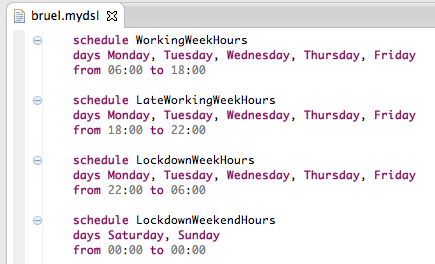
\includegraphics[width=10cm]{dsl-schedules.png}
	\caption{An example of \textit{schedules} defined for a interviewee.}
	\label{fig:dsl-schedules}
\end{figure}

\newpage
\subsection{Building specification}\label{subsec:buildingspecification}
Rooms and room types are part of the complete building specification, with terminology rooted in concepts revolving around buildings, ie. rooms, room types, floors, different sensors and actuators. \\

To avoid confusing the DSL user with an overwhelming amount of declarations of rooms, sensors and actuators - we have designed \textit{room types} that declare static use of sensors and actuators. Independent rooms that stick out from the crown can still be defined on an instance level.

\begin{figure}
  \centering
    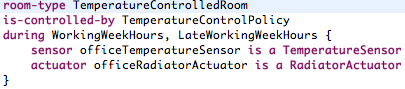
\includegraphics[width=10cm]{dsl-room-types.png}
	\caption{An example of \textit{room types} defined for a interviewee.}
	\label{fig:room-types}
\end{figure}

\newpage
Building specification as in the example below, helps us map out the actual buildings as they are in our DSL. With this we are able to accurately define exact locations for sensors and actuators as well as implement policies for rooms in specific locations. 

\begin{figure}
  \centering
	 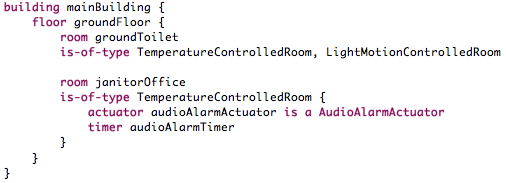
\includegraphics[width=10cm]{dsl-building-definition.png}  
	\caption{An example of \textit{building specification} defined for a interviewee.}
	\label{fig:dsl-building-definition}
\end{figure}

\newpage
\subsection{Policy}\label{subsec:policies}
Policies define the actual behavior, ie. adjustment of actuators, based on sensor input. 

\begin{figure}
  \centering
    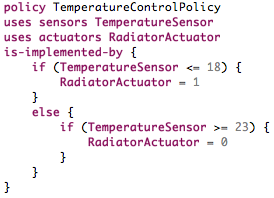
\includegraphics[width=10cm]{dsl-policy-definition.png} 
	\caption{An example of \textit{policy definition} defined for a interviewee.}
	\label{fig:dsl-policy-definition}
\end{figure}

\newpage
\section{Evaluation}\label{sec:evaluation}

\subsubsection{Br\"{u}el \& Kj\ae r}\label{subsec:bruel}
The requirements received from Br\"{u}el \& Kj\ae r were implemented in our DSL and can be found in \nameref{sec:dsl-bruel}. One of the requirements from the interview (\textit{all sensor and actuator data stored in a repository for use in a visual display of data in the FM office}) was not implemented in our DSL because we decided to narrow the scope of the project. After evaluating these requirements, we realized that some of the sensors and actuators needed to satisfy the implementation are not defined in our metamodel. While these problems could be easily fixed by simply adding some new classes in the metamodel, we evaluated this area as one that our DSL can be further improved as discussed in \nameref{subsec:def-sensor-actuator-types}.


\subsubsection{Bygningstyrelsen}\label{subsec:bygstyrelsen}
TO BE EVALUATED

\subsubsection{K\o benhavns Tekniske Skole}\label{subsec:kts}
The implementation of these requirements in our DSL can be found in \nameref{sec:dsl-kts} and just like in the evaluation in \nameref{subsec:bruel}, we faced the same lack of sensors and actuators. This seems to be a recurring issue in our language but nonetheless it provides a nice opportunity to improve our language. It is further discussed in \nameref{subsec:def-sensor-actuator-types}. 
Another aspect of our language that can be refined is the ability to define how each policy should be used as discussed in \nameref{subsec:during}. 
 
\subsubsection{UNI-C}\label{subsec:uni-c}
TO BE EVALUATED

\section{Discussion}\label{sec:discussion}
\subsection{Future Work}\label{subsec:futurework}

\subsubsection{Graphical Editor for policy definition}\label{subsec:graphicaleditor}
Our DSL editor is text based and most of the keywords we have chosen to use are words commonly used in the industry. In the way they are structured and used in our DSL, they literally describe the meaning of the combined keywords. The textual editor is sufficient in all definitions but in the policy definition one needs to have some programming knowledge in order to understand and know how to use the expression language. Therefore, in order to accommodate the normal users and give them a superior user experience, improvement of our DSL is necessary by developing a graphical editor for the policies to abstract the expression language and consequently make it simpler for users to define them.

\subsubsection{Integration with existing systems}\label{subsec:integration}
In our metamodel, we have included some external systems that already exist; (\textit{CTS, Access Control, Calender System and Meeting Shedule Systems}) and used in some buildings. Those systems are usually closed, proprietary systems. Some form of integration is possible to some of them, but would need to be evaluated case by case. The (\textit{CTS}) is somewhat advanced and needs thorough knowledge of the tool to properly use it. The GUI looks like an electrical diagram, and is not made for ease of use. Moreover, the temperatures shown in the program are from sensors in the ventilation ducts, not in the room themselves, adding extra complexity. As it is today, it is not really possible to integrate CTS systems into custom made solutions, like our DSL, since they are proprietary systems and guarded well in order to sell service packages to the users.

\subsubsection{Enhanced Code Completion}\label{subsec:codecompletion}
Code completion is of great importance to our language because it really helps the user by guiding her in all possible options she has. Right now our DSL has an up-and-running code completion but in the future we would like to restrict it in a way that only the declared/defined elements should be available. In \nameref{fig:code-completion} below, we present our DSL as it currently is but if restricted, should only be able to provide TemperatureSensor and RadiatorActuator as options for the TemperatureControlPolicy to the user.

\begin{figure}
  \centering
    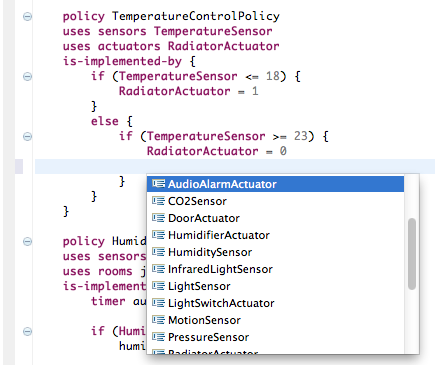
\includegraphics[width=10cm]{dsl-code-completion.png} 
	\caption{An example of \textit{code completion}.}
	\label{fig:code-completion}
\end{figure}

\subsubsection{Defining Actuator and Sensor types}\label{subsec:def-sensor-actuator-types}
From the evaluation section above, we came to realize that some of the sensors and actuators needed to satisfy the requirements are not implemented in our DSL. A quick fix would be to add them to our metamodel but this still will not give us the flexibility to define policies using actuators and sensors that are not available in our DSL when needed. Future work in this area might include a minor modification of our DSL in order to accommodate definition of actuators and sensors as needed. Sort of the same concept as the predefined room types. This flexibility will make our DSL more adaptable.


\subsubsection{Time Loop}\label{subsec:looptime}
Our loop is based on an outer loop that calls all policies in every iteration. In the future it could be based on a prioritization of room, room-type or policies adding extra flexibility and fine grained control to the language. For instance, specify that some policies should only run once in an hour.

\subsubsection{When to run policies}\label{subsec:during}
In its current state, our DSL allows us to determine when the policies should be run by using the already defined schedules. One or more policies can be run based on one or more schedules. As shown in the image below, we specify a schedule for all governing policies of that room-type. 
\begin{figure}
  \centering
    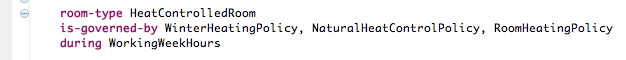
\includegraphics[scale=0.5]{dsl-during.png} 
	\caption{An example to \textit{during} when using policies in rooms.}
	\label{fig:during}
\end{figure}
In case we have several governing policies that run on different schedules, our DSL does not allow us to assign a specific schedule to every single governing policy. An interesting improvement that could increase our DSL's flexibility would be the ability to specify a different schedule for each of the policies governing a room. 

\section{Conclusion}\label{sec:conclusion}
In our point of view, the proposed DSL constitutes a useful tool to every simple user planning to define automation policies for his residence or working place. The supporting arguments are the user-friendly interface and the self-explanatory keywords alongside with the flexibility of the abstraction that the DSL provides. Naturally, its scope is narrowed and there is no actual implementation yet, mainly due to the size of the team and the limitations of the semester, but nevertheless it can potentially be improved in many ways as described in ~\nameref{sec:discussion} and lead to the development of an energy-efficient ally of our welfare in both a personal and global dimension. 

\bibliography{BPE}{}
\bibliographystyle{plain}

\section{Appendix A - DSL MetaModel}
The complete Ecore MetaModel can be viewed online at
\url{https://github.com/rugbroed/BPE/blob/Version-0.9/documents/ecore-policy-engine.png}

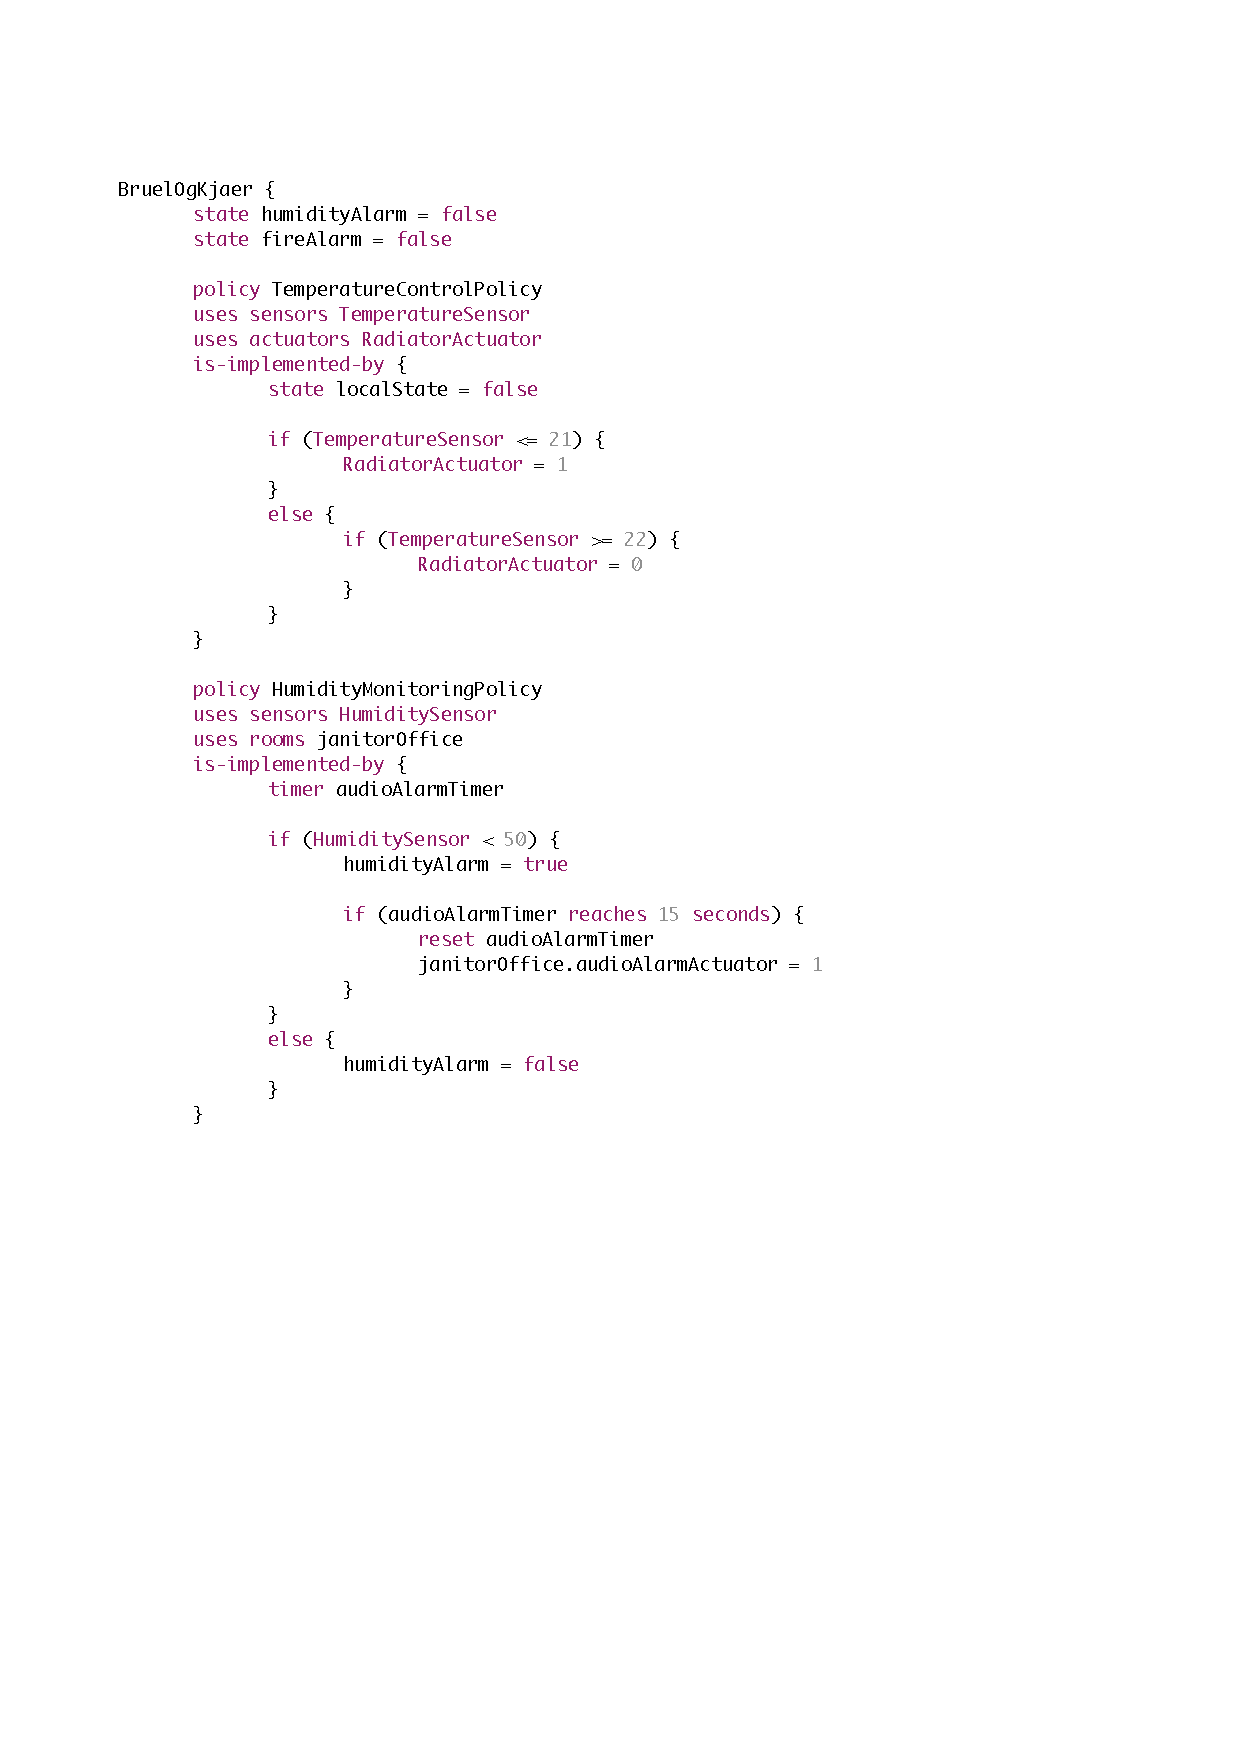
\includepdf[pages=1,scale=.8,pagecommand=\section{Appendix B - Br\"{u}el \& Kj\ae r}]{BruelOgKjaer.pdf}
\includepdf[pages=2-,scale=.8,pagecommand={}]{BruelOgKjaer.pdf}

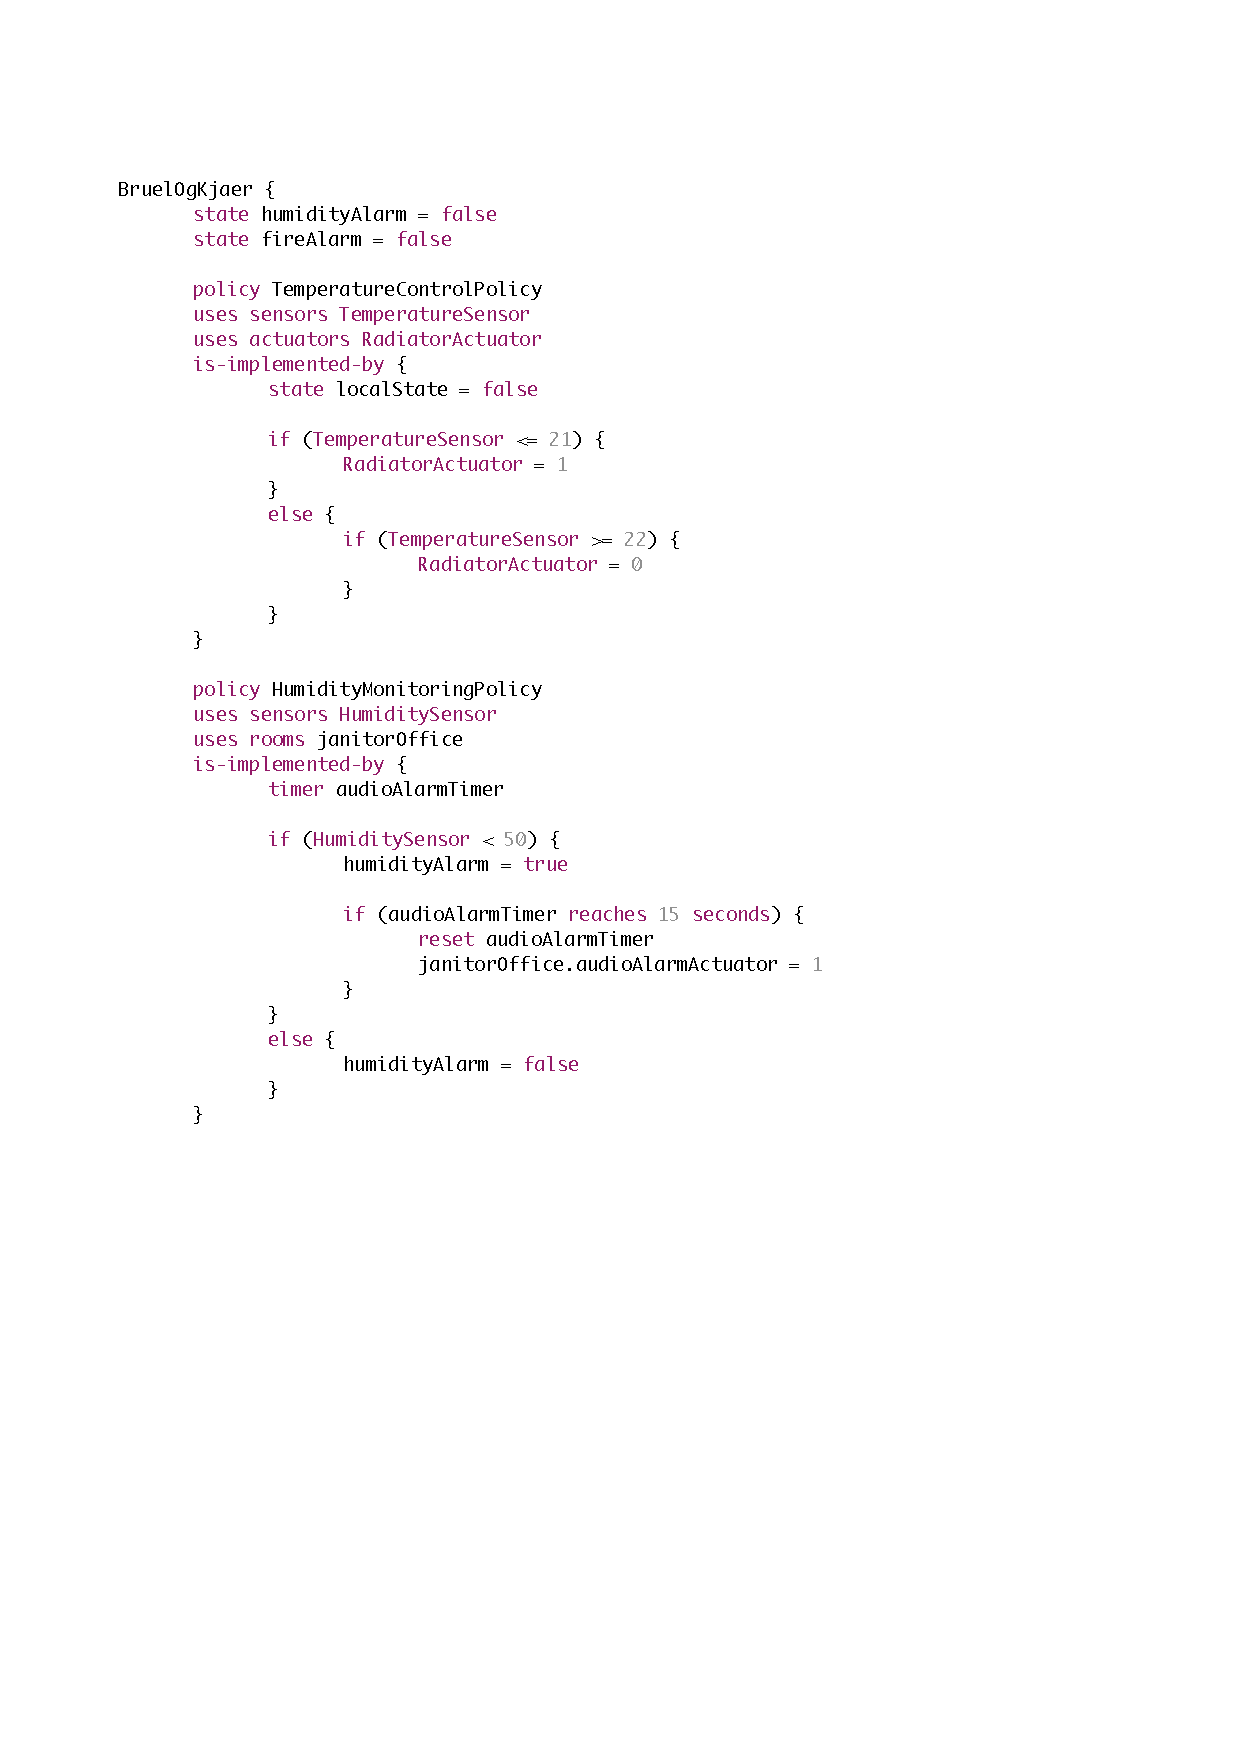
\includepdf[pages=1,scale=.8,pagecommand=\section{Appendix C - DSL for K\o benhavns Tekniske Skole}\label{sec:bygningsstyrelsen}]{BruelOgKjaer.pdf}
\includepdf[pages=2-,scale=.8,pagecommand={}]{BruelOgKjaer.pdf}

\end{document}